% Provenance (never printed): old seconde/premiere S material on the water
% cycle on land (the drainage basin, river discharge, floods and their
% management); see sources/book2/PROVENANCE.md. The Varden basin is computed
% in figdata/grade-10/varden_basin.py from figdata/shared/region.py; the
% Potomac record in figdata/grade-10/flood_frequency.py.
\chapter{أحواض التصريف والأنهار والفيضانات}\label{ch:g10:drainage-basins}

قد يرتفع نهر بعد يومين من توقف المطر، عند بلدة لم يسقط فيها مطر قط. فالماء الذي
يغمر شوارعها سقط قبل ذلك، على تلال بعيدة في أعلى المجرى؛ وانحدر على سفوحها إلى
الجداول، والتقت الجداول في النهر الذي جلبه، دفعة واحدة، إلى البلدة. ولفهم فيضان،
يجب أن ننظر إلى ما وراء النهر، إلى المساحة كلها التي تغذيه، وأن نتتبع الماء عبرها.
يعرّف هذا الفصل تلك المساحة، \omterm{def:g10:drainage-basins:drainage-basin}{حوض التصريف}؛ ويقيس ما يحمله النهر، تصريفه؛ ويتتبع
فيضانًا وهو يمر بنقطة من النهر؛ ويبيّن كيف يخبرنا سجل طويل من الفيضانات بعدد المرات
التي يعود فيها فيضان معين.

\begin{omfigure}
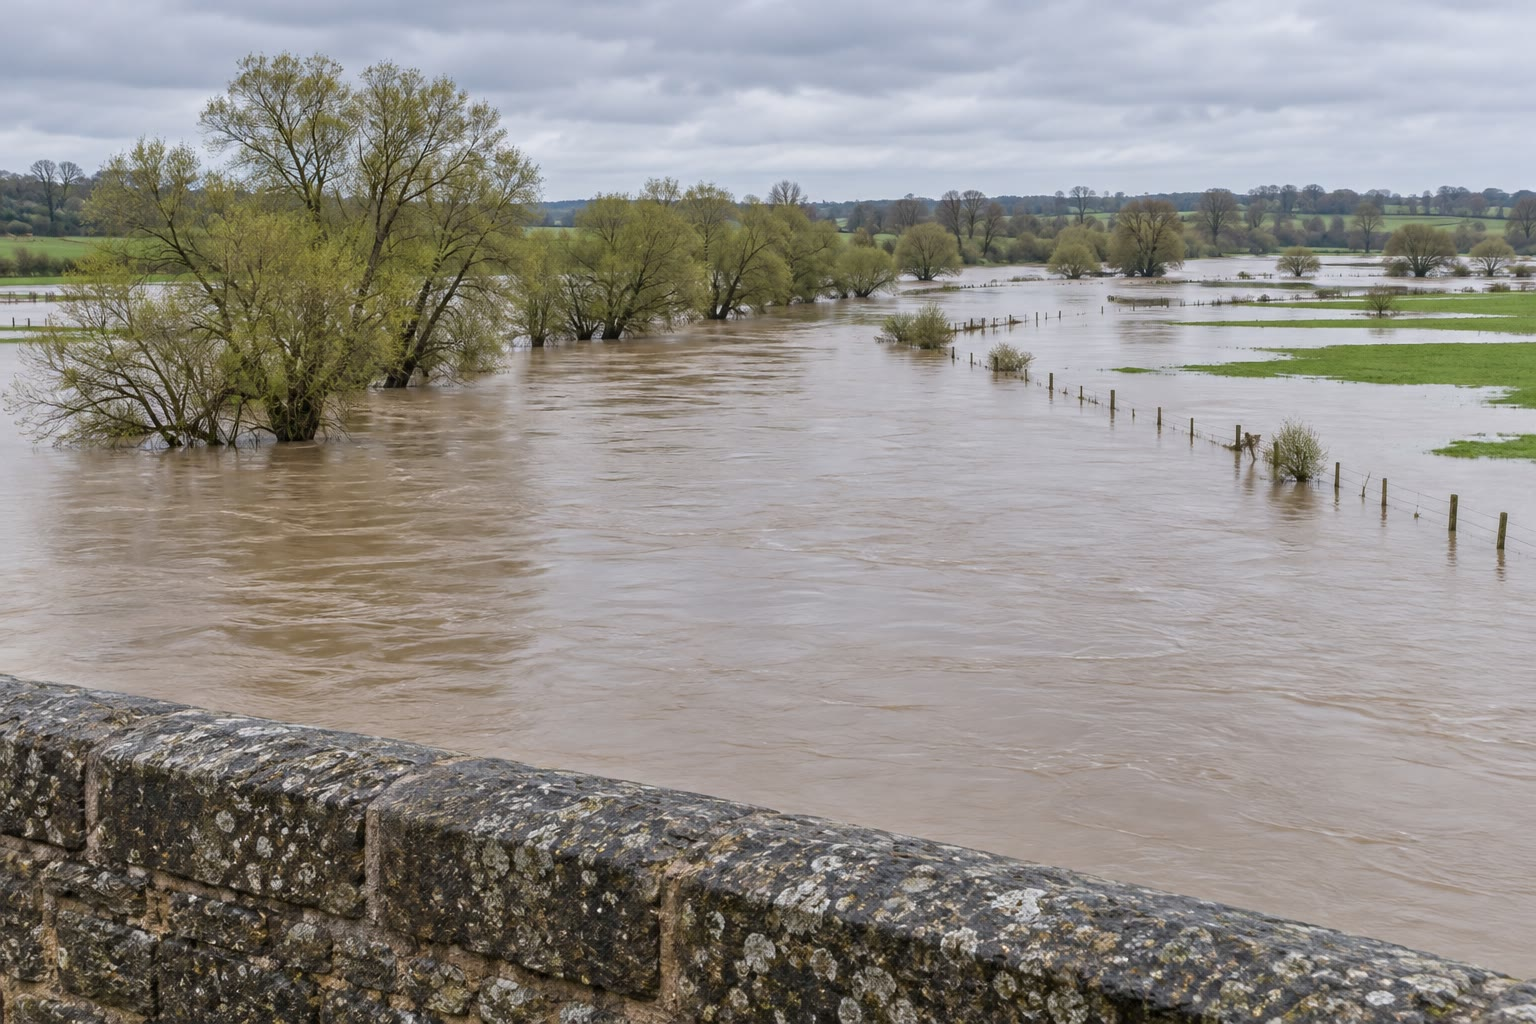
\includegraphics[width=0.8\linewidth]{images/book2/ai/g10-river-flood-meadows.jpg}

{\small نهر في فيضان، كما يُرى من جسر حجري: الماء البني، المحمّل بالطمي، غادر مجراه
وغطى مروج سهله الفيضي، حتى الأسوار والأشجار التي تحف بضفتيه
المعتادتين.}
\end{omfigure}

\begin{recall}
المطر الذي يبلغ الأرض يتسرب فيها، أو يجري على سطحها، أو يتبخر؛ والدورة المائية
تعيده إلى البحر (كتب الفيزياء). ويتسرب الماء في الصخور النفوذة ويملؤها تحت منسوب
المياه الجوفية، مكوّنًا طبقات حاملة للمياه تغذي الينابيع والأنهار (الكتاب 1،
الصف 6). ويتعرج النهر في منعطفات عبر سهله الفيضي المنبسط، الذي يغطيه حين يفيض
(الكتاب 1، الصف 5). وتصل خطوط الكنتور بين نقاط متساوية
الارتفاع؛ وتلال فاردن هي المنطقة المرسومة على خرائط هذه السلسلة
(الكتاب 1، الصفان 2 و9).
\end{recall}

\begin{safety}
ماء الفيضان أخطر بكثير مما يبدو. فنحو \qty{15}{cm} من الماء السريع الجريان قد
تُسقط شخصًا بالغًا، ونحو \qty{30}{cm} قد تجرف سيارة؛ والطريق تحته ربما انهار. لا
تمشِ أبدًا في ماء الفيضان ولا تقد سيارتك فيه: استدر واسلك طريقًا
آخر.
% ledger: nws:flood-water
\end{safety}

\section{حوض التصريف}

كل قطرة مطر لا تتبخر ولا تتسرب عميقًا تجري نحو الأسفل. فهي تتبع أشد انحدار للأرض،
وتنضم إلى مسيل، ثم إلى جدول، وتلتقي الجداول في أنهار. والأرض كلها التي ينتهي
ماؤها في النهر نفسه تكوّن وحدة واحدة.

\begin{definition}[حوض التصريف؛ خط تقسيم المياه]\label{def:g10:drainage-basins:drainage-basin}
\emph{حوض التصريف}\index{حوض التصريف} لنقطة من نهر هو المساحة كلها من الأرض التي
يجري ماؤها السطحي إلى النهر في أعلى تلك النقطة ويمر بها. و\emph{خط تقسيم
المياه}\index{خط تقسيم المياه} هو الخط الذي يفصل بين حوضَي \omterm{def:g10:drainage-basins:discharge}{تصريف} متجاورين: يتبع
قمم الأرض، والمطر الساقط على أي من جانبيه يجري إلى أنهار
مختلفة.
\end{definition}

يُعرَّف الحوض دائمًا لنقطة من النهر، هي \emph{مخرجه}: فحوض النهر عند بلوغه البحر
هو الأكبر، ولكل نقطة في أعلى المجرى حوض أصغر داخله. وقطرتان تسقطان على بعد متر
واحدة من الأخرى، على جانبي خط تقسيم، قد تنتهيان في نهرين مختلفين بل في محيطين
مختلفين.

\subsection*{حوض نهر فاردن}

يجد الحاسوب \omterm{def:g10:drainage-basins:drainage-basin}{حوض التصريف} من خريطة ارتفاعات في خطوات قليلة. فتُقسم الخريطة إلى مربعات
صغيرة، طول ضلعها هنا \qty{50}{m}. ولكل مربع، ينظر الحاسوب في جيرانه الثمانية ويرسل
الماء إلى الجار الذي يُبلغ بأشد انحدار نازل. (وحيث لا يكون لمنخفض صغير جار أدنى،
يُملأ أولًا حتى المستوى الذي يفيض عنده، كما تفعل البركة.) واتباع هذه الخطوات من مربع
إلى مربع يرسم مسار قطرة من أي مكان على الخريطة. والمربعات التي تبلغ قطراتها النهر
تكوّن الحوض.

\begin{omfigure}
\begin{tikzpicture}
\begin{axis}[axis equal image, xmin=0, xmax=10, ymin=0, ymax=8, width=0.86\linewidth,
  tick label style={font=\scriptsize}, xlabel={\foreignlanguage{arabic}{الشرق \babelsublr{(km)}}}, ylabel={\foreignlanguage{arabic}{الشمال \babelsublr{(km)}}},
  label style={font=\small}, enlargelimits=false]
\addplot[fill=omDef!14, draw=none, even odd rule] table {figdata/out/grade-10-varden_basin-fill.dat};
\addplot[contour, line width=0.25pt, opacity=0.7] table {figdata/out/shared-region-contours.dat};
\addplot[index contour, opacity=0.8] table {figdata/out/shared-region-index-contours.dat};
\addplot[river, line width=1.6pt] table {figdata/out/shared-region-river.dat};
\addplot[omThm, line width=1.4pt, dashed] table {figdata/out/grade-10-varden_basin-divide.dat};
\addplot[omWxRain, line width=0.9pt, -{Stealth[length=5pt]}] table {figdata/out/grade-10-varden_basin-path1.dat};
\addplot[omWxRain, line width=0.9pt, -{Stealth[length=5pt]}] table {figdata/out/grade-10-varden_basin-path2.dat};
\addplot[omWxRain, line width=0.9pt, -{Stealth[length=5pt]}] table {figdata/out/grade-10-varden_basin-path3.dat};
\addplot[omWxRain, line width=0.9pt, -{Stealth[length=5pt]}] table {figdata/out/grade-10-varden_basin-path4.dat};
\fill[omWxRain] (axis cs:2,7.4) circle (2.2pt);
\fill[omWxRain] (axis cs:4,1.8) circle (2.2pt);
\fill[omWxRain] (axis cs:8.6,6.6) circle (2.2pt);
\fill[omWxRain] (axis cs:2.5,0.7) circle (2.2pt);
\node[font=\footnotesize, fill=white, fill opacity=0.85, text opacity=1, inner sep=1.5pt, text=omThm] at (axis cs:6.0,6.75) {خط التقسيم};
\node[font=\footnotesize, fill=white, fill opacity=0.85, text opacity=1, inner sep=1.5pt, text=omThm] at (axis cs:3.5,1.1) {خط التقسيم};
\node[font=\footnotesize, fill=white, fill opacity=0.85, text opacity=1, inner sep=1.5pt, align=center] at (axis cs:5.3,7.55) {\foreignlanguage{arabic}{خارج الحوض:}\\الماء يغادر نحو الشمال};
\node[font=\footnotesize, fill=white, fill opacity=0.85, text opacity=1, inner sep=1.5pt, align=right, anchor=east] at (axis cs:9.85,3.35) {المخرج};
\draw[-{Stealth[length=6pt]}, line width=1pt, omRiver] (axis cs:9.3,3.7) -- (axis cs:9.95,4.15);
\node[font=\footnotesize, fill=white, fill opacity=0.85, text opacity=1, inner sep=1.5pt] at (axis cs:1.1,4.75) {النهر};
\end{axis}
\end{tikzpicture}

{\small حوض \omterm{def:g10:drainage-basins:discharge}{تصريف} نهر فاردن على خريطة تلال فاردن (مظلل)، محسوب بإرسال ماء كل مربع
طول ضلعه \qty{50}{m} على أشد انحدار؛ وخطوط الكنتور كل \qty{50}{m}. والخطوط
المتقطعة هي خطوط التقسيم؛ والخطوط الزرقاء مسارات أربع قطرات مطر (النقاط).
تبلغ اثنتان منها النهر وتجريان شرقًا إلى المخرج، حيث يغادر النهر الخريطة؛ والأخريان،
وراء خطوط التقسيم، تغادران الخريطة نحو أنهار
أخرى.}
\end{omfigure}

يغطي الحوض \qty{66}{km^2} من مساحة الخريطة البالغة \qty{80}{km^2}، أي نحو
أربعة أخماسها. وفي الشمال يتبع خط التقسيم قمم التلال ويمر فوق ذراها؛ ووراءها تنحدر
الأرض بعيدًا عن النهر ويجري ماؤها إلى وادٍ آخر. وفي الركن الجنوبي الغربي تصرف مساحة
صغيرة ماءها أيضًا خارج الخريطة. والنهر نفسه يدخل الخريطة من الغرب، فحوضه الكامل
أكبر: إذ يشمل أيضًا الأرض الواقعة في أعلى المجرى، وراء حافة
الخريطة.
% values computed in figdata/grade-10/varden_basin.py (basin_km2 66.19, map_km2 80)

\subsection*{أكبر الأنهار}

تُقارن الأنهار بمساحة أحواضها وبالماء الذي تحمله. وأكبر نهر في العالم بفارق كبير هو
الأمازون. أما المسيسيبي، أكبر أنهار الولايات المتحدة، فيصرّف نحو \num{1150000}
ميل مربع، أي نحو 2.98 مليون \unit{km^2}، من الولايات المتحدة
وكندا.
% ledger: kammerer:mississippi

\section{التصريف}

\begin{definition}[التصريف]\label{def:g10:drainage-basins:discharge}
\emph{التصريف}\index{تصريف} لنهر عند نقطة هو حجم الماء الذي يعبر مقطعًا عرضيًا
للنهر في ثانية واحدة. ويُقاس بالأمتار المكعبة في الثانية،
\unit{m^3/s}.
\end{definition}

\omterm{def:g10:drainage-basins:discharge}{تصريف} قدره \qty{1}{m^3/s} هو ألف لتر في كل ثانية، أو
\qty{86400}{m^3} في اليوم. ويجري الماء أسرع ما يكون قرب السطح في وسط المجرى وأبطأ ما
يكون على امتداد قاعه وضفتيه، حيث يحتك بهما؛ و\emph{السرعة المتوسطة} هي السرعة
المتوسطة على المقطع العرضي
كله.

\begin{proposition}[التصريف والسرعة والمقطع العرضي]\label{prop:g10:drainage-basins:discharge}
\omterm{def:g10:drainage-basins:discharge}{تصريف} النهر $Q$ هو جداء السرعة المتوسطة $v$ للماء ومساحة $A$ المقطع العرضي
المبلول:
\[
Q = v\,A.
\]
\end{proposition}

\begin{proof}
في زمن $t$، يكون الماء الذي يعبر المقطع قد تقدم مسافة
$v\,t$: فهو يملأ شريحة من النهر مقطعها العرضي $A$ وطولها
$v\,t$، وحجمها $A\,v\,t$. وقسمة هذا الحجم على الزمن $t$
تعطي الحجم في الثانية، $Q = v\,A$.
\end{proof}

نهر مقطعه العرضي \qty{50}{m^2} يجري بسرعة متوسطة قدرها
\qty{1.2}{m/s} يحمل $1.2 \times 50 = \qty{60}{m^3/s}$. وفي الفيضان يكبر العاملان
كلاهما: يعمق الماء ويتسع، فيكبر المقطع العرضي، ويجري
أسرع.

\subsection*{قياس التصريف}

لما كانت السرعة تتغير عبر النهر، فإنها تُقاس في عدة نقاط. فيُقسم النهر إلى شرائح
رأسية؛ وفي كل منها يُقاس العمق والسرعة، وتُجمع تصريفات
الشرائح.

\begin{method}[طريقة السرعة والمساحة]\label{met:g10:drainage-basins:velocity-area}
\begin{enumerate}
  \item مُدّ شريط قياس عبر النهر واختر عليه خطوطًا رأسية بفواصل منتظمة
        $w$.
  \item عند كل خط رأسي، قِس العمق $d$ والسرعة المتوسطة $v$
        للماء على ذلك العمق بمقياس التيار.
  \item يمثل كل خط رأسي شريحة عرضها $w$ ومساحتها $w\,d$؛ وتصريفها
        $v\,w\,d$.
  \item اجمع تصريفات الشرائح كلها: $Q = \sum v\,w\,d$.
        والمقطع العرضي $A = \sum w\,d$ والسرعة المتوسطة $Q/A$.
\end{enumerate}
\end{method}

\begin{omfigure}
\begin{tikzpicture}[x=0.9cm, y=1.6cm, font=\footnotesize]
  % water
  \fill[omSea] (0,0) -- (1,-0.4) -- (2,-0.75) -- (3,-1.0) -- (4,-1.25) -- (5,-1.4) -- (6,-1.3)
     -- (7,-1.1) -- (8,-0.8) -- (9,-0.5) -- (10,-0.2) -- (10.5,0) -- cycle;
  \fill[omDef!22] (4,0) -- (4,-1.25) -- (5,-1.4) -- (6,-1.3) -- (6,0) -- cycle;
  % bed
  \draw[line width=0.9pt, brown!60!black] (-0.6,0.35) -- (0,0) -- (1,-0.4) -- (2,-0.75) -- (3,-1.0) -- (4,-1.25)
     -- (5,-1.4) -- (6,-1.3) -- (7,-1.1) -- (8,-0.8) -- (9,-0.5) -- (10,-0.2) -- (10.5,0) -- (11.1,0.35);
  \draw[omDef!70!black, line width=0.5pt] (0,0) -- (10.5,0);
  % verticals
  \foreach \x/\d/\v/\dx in {1/0.4/0.3/0.3, 3/1.0/0.6/0, 5/1.4/0.8/0, 7/1.1/0.7/0, 9/0.5/0.4/-0.25} {
    \draw[black!70, dashed] (\x,0) -- (\x,-\d);
    \node[anchor=south, font=\scriptsize] at (\x,0.02) {\qty{\v}{m/s}};
    \node[font=\scriptsize, fill=white, inner sep=0.8pt] at (\x+\dx,-0.5*\d) {\qty{\d}{m}};
  }
  \draw[{Stealth}-{Stealth}] (4,0.42) -- node[above, font=\scriptsize] {\foreignlanguage{arabic}{شريحة واحدة: $w = \qty{2}{m}$}} (6,0.42);
  \node[anchor=west, align=left] at (11.2,-0.15) {سطح\\الماء};
  \node[anchor=west, align=left] at (11.2,-0.9) {القاع};
  \draw[black!50] (11.15,-0.9) -- (8.5,-0.68);
  \node[anchor=north] at (5.25,-1.75) {السرعات المتوسطة المقيسة عند الخطوط الرأسية فوق الماء، والأعماق في الماء};
\end{tikzpicture}

{\small قياس \omterm{def:g10:drainage-basins:discharge}{تصريف} (رسم تخطيطي؛ والمقياس الرأسي مبالغ فيه). خمسة خطوط رأسية،
بين كل منها والآخر \qty{2}{m}، تقسم جدولًا عرضه نحو \qty{10}{m} إلى
شرائح؛ والشريحة المظللة هي التي قيست عند الخط الرأسي الأوسط.}
\end{omfigure}

\begin{example}[قياس التصريف]\label{ex:g10:drainage-basins:gauging}
في جدول الشكل، مساحات الشرائح الخمس، وعرض كل منها \qty{2}{m}، هي
$2 \times 0.4 = 0.8$ و$2.0$ و$2.8$ و$2.2$ و\qty{1.0}{m^2}: فالمقطع
العرضي \qty{8.8}{m^2}. وتصريفاتها $0.3 \times 0.8 =
0.24$ و$0.6 \times 2.0 = 1.20$ و$0.8 \times 2.8 = 2.24$ و$0.7 \times 2.2 =
1.54$ و$0.4 \times 1.0 = \qty{0.40}{m^3/s}$، فالجدول يحمل
$Q \approx \qty{5.6}{m^3/s}$. والسرعة المتوسطة $5.62/8.8 \approx
\qty{0.64}{m/s}$، أي أقل من \qty{0.8}{m/s} في وسط الجدول.
\end{example}

\begin{omfigure}
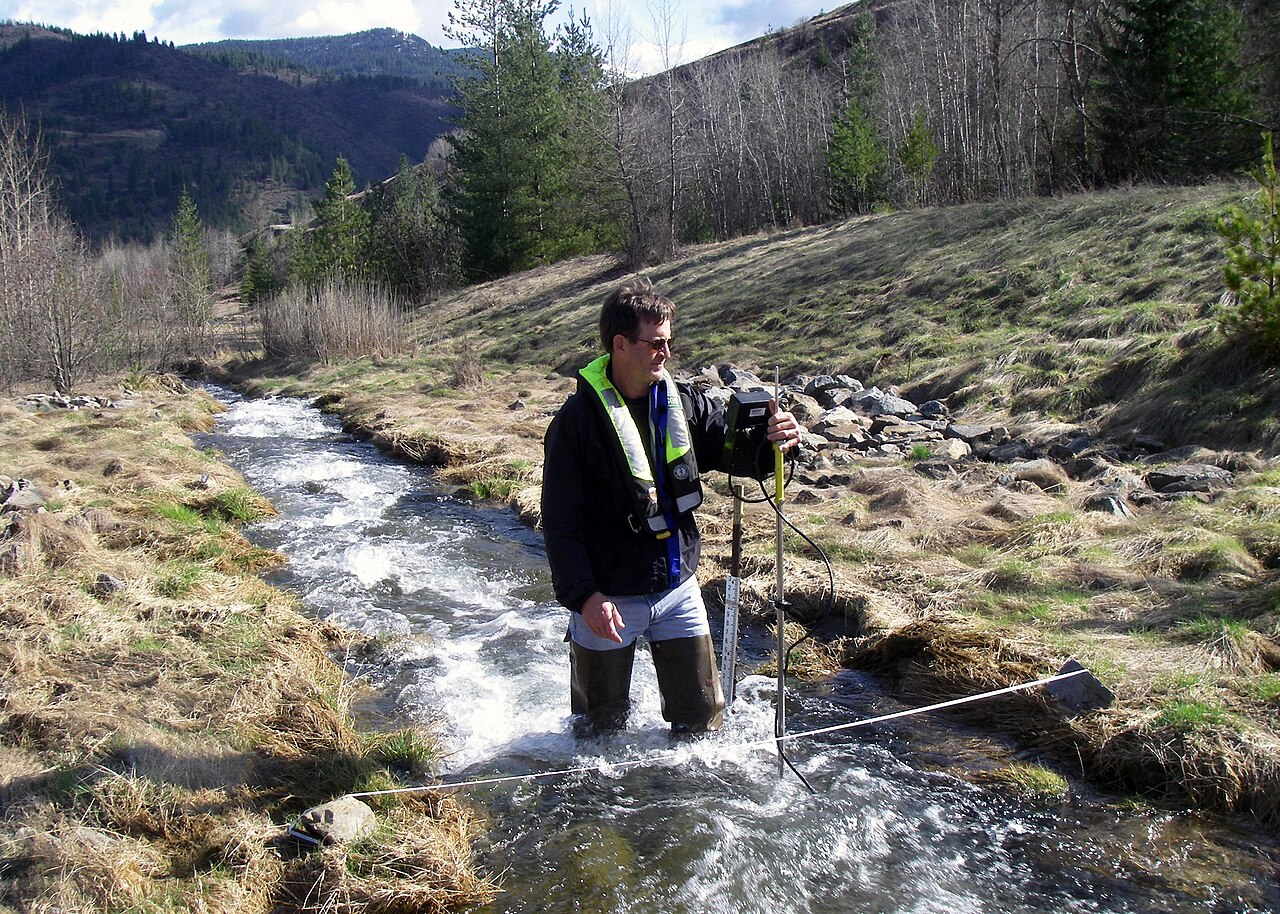
\includegraphics[height=4.6cm]{images/book2/g10-usgs-hydrologist-streamflow.jpg}\hspace{0.3cm}%
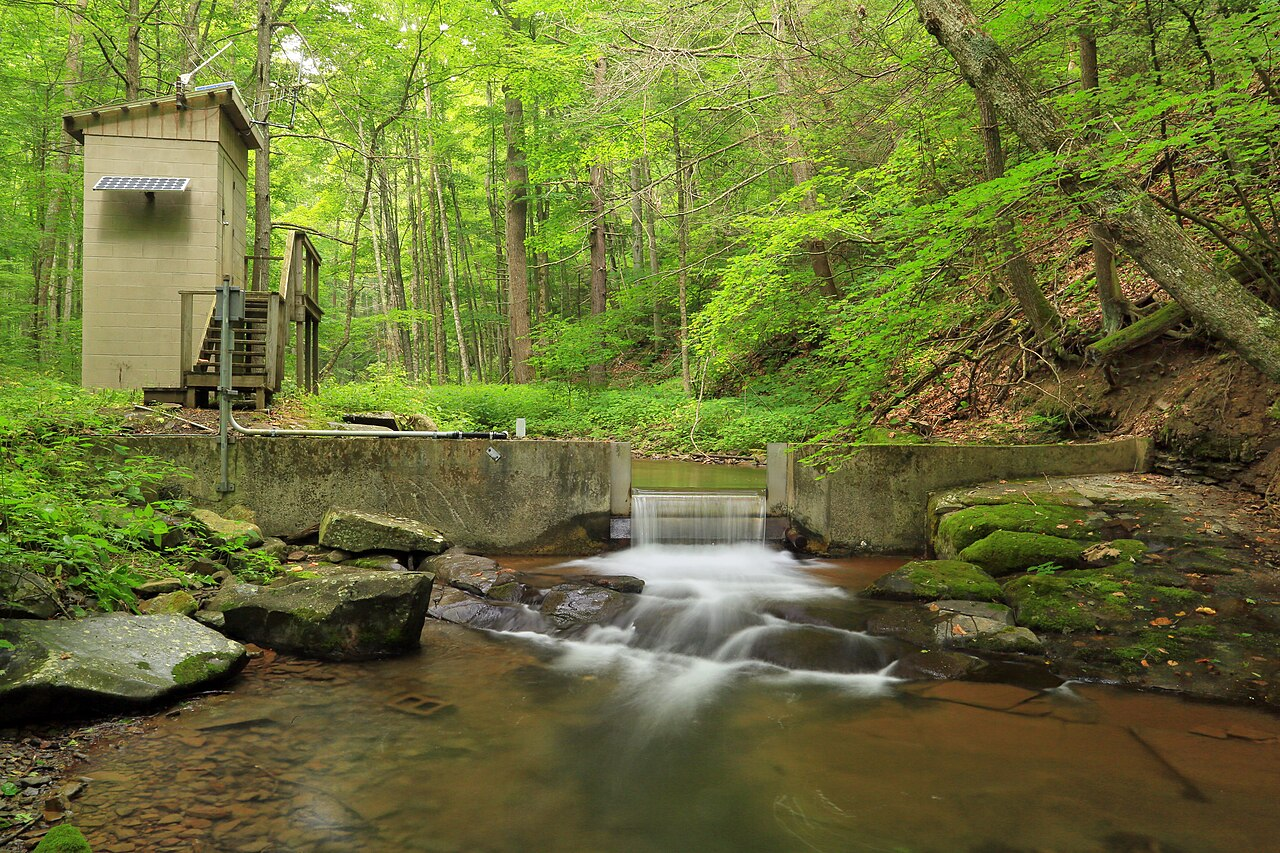
\includegraphics[height=4.6cm]{images/book2/g10-usgs-streamgage.jpg}

{\small في اليمين: عالم هيدرولوجيا يقيس \omterm{def:g10:drainage-basins:discharge}{تصريف} جدول جبلي بطريقة السرعة
والمساحة؛ والشريط الممدود عبر الجدول يحدد الخطوط الرأسية، والقضيب يحمل مقياس
التيار. في اليسار: محطة قياس على جدول في غابة؛ ويضم الكوخ الأجهزة التي تسجل منسوب
الماء خلف الهدّار الصغير. الصور: هيئة المسح الجيولوجي الأمريكية
(ملك عام).}
\end{omfigure}

قياس \omterm{def:g10:drainage-basins:discharge}{التصريف} يستغرق وقتًا ولا يمكن إجراؤه باستمرار. لذلك تسجل محطة القياس
منسوب الماء، دون انقطاع. وتعطي بضعة قياسات \omterm{def:g10:drainage-basins:discharge}{للتصريف} أُجريت عند مناسيب مختلفة
منحنى يربط المنسوب \omterm{def:g10:drainage-basins:discharge}{بالتصريف}، فتحوّل المحطة كل منسوب تسجله إلى
\omterm{def:g10:drainage-basins:discharge}{تصريف}.

تحمل الأنهار الكبرى تصريفات هائلة. فمن 1972 إلى 2003 صبّ الأمازون في المحيط
الأطلسي في المتوسط نحو \qty{206000}{m^3/s}، بدقة قرابة
\qty{6}{\percent}: أي نحو \qty{17}{\percent} من كل الماء العذب الذي تجلبه
أنهار العالم إلى البحر. ويجلب المسيسيبي في المتوسط
\num{593000} قدم مكعب في الثانية، أي نحو \qty{16800}{m^3/s}، إلى خليج
المكسيك: فالأمازون يحمل نحو اثني عشر ضعفًا من ذلك.
% ledger: callede:amazon, kammerer:mississippi

\section{الهيدروغراف}

\begin{definition}[الهيدروغراف؛ التدفق القاعدي؛ زمن التأخر]\label{def:g10:drainage-basins:hydrograph}
\emph{الهيدروغراف}\index{هيدروغراف} هو منحنى \omterm{def:g10:drainage-basins:discharge}{تصريف} نهر عند نقطة واحدة بدلالة
الزمن. و\emph{التدفق القاعدي}\index{تدفق قاعدي} هو جزء \omterm{def:g10:drainage-basins:discharge}{التصريف} الذي تغذيه المياه
الجوفية، والذي يبقي النهر جاريًا بين الأمطار. و\emph{زمن التأخر}\index{زمن التأخر}
لفيضان هو الزمن بين ذروة الهطول على الحوض وذروة
\omterm{def:g10:drainage-basins:discharge}{التصريف}.
\end{definition}

\begin{omfigure}
\begin{tikzpicture}[x=1cm, y=1cm, font=\footnotesize]
  \draw[-{Stealth}] (0,0) -- (10.2,0) node[below left] {الزمن};
  \draw[-{Stealth}] (0,0) -- (0,5.9) node[above right] {التصريف};
  % rain bars hanging from the top
  \draw[black!50] (0,5.4) -- (10,5.4);
  \foreach \x/\h in {1.0/0.15, 1.3/0.35, 1.6/0.55, 1.9/0.4, 2.2/0.2} {
    \fill[omWxRain!70] (\x,5.4) rectangle ++(0.28,-\h);
  }
  \node[anchor=south west] at (2.6,5.4) {الهطول على الحوض};
  % baseflow and hydrograph
  \fill[omSea] (0,0.7) -- (2.0,0.7) .. controls (2.8,0.8) and (3.3,3.3) .. (4.0,3.6)
    .. controls (4.6,3.6) and (5.1,2.1) .. (6.0,1.55) .. controls (7.0,1.0) and (8.0,0.85) .. (10,0.8)
    -- (10,0) -- (0,0) -- cycle;
  \fill[omLithAlluv] (0,0) -- (0,0.7) -- (2.0,0.7) .. controls (3.5,0.68) and (5.5,0.75) .. (6.6,0.95)
    .. controls (8,1.0) and (9,0.85) .. (10,0.8) -- (10,0) -- cycle;
  \draw[omDef, line width=1.2pt] (0,0.7) -- (2.0,0.7) .. controls (2.8,0.8) and (3.3,3.3) .. (4.0,3.6)
    .. controls (4.6,3.6) and (5.1,2.1) .. (6.0,1.55) .. controls (7.0,1.0) and (8.0,0.85) .. (10,0.8);
  \draw[black!60, dashed] (2.0,0.7) .. controls (3.5,0.68) and (5.5,0.75) .. (6.6,0.95);
  % lag time
  \draw[black!60, densely dotted] (1.74,4.85) -- (1.74,4.3);
  \draw[black!60, densely dotted] (3.98,3.65) -- (3.98,4.3);
  \draw[{Stealth}-{Stealth}] (1.74,4.3) -- node[above] {زمن التأخر} (3.98,4.3);
  % labels
  \node[anchor=west] at (4.2,3.75) {الذروة};
  \node[anchor=east, align=right] at (2.9,2.2) {الطرف\\الصاعد};
  \node[anchor=west, align=left] at (5.4,2.3) {الطرف الهابط};
  \node[align=center] at (4.5,1.25) {الجريان السطحي};
  \node at (8.2,0.4) {التدفق القاعدي};
\end{tikzpicture}

{\small \omterm{def:g10:drainage-basins:hydrograph}{هيدروغراف} فيضان (رسم تخطيطي). بعد المطر، يرتفع \omterm{def:g10:drainage-basins:discharge}{التصريف} إلى ذروة ثم ينخفض
عائدًا ببطء أكبر؛ والمساحة تحت المنحنى هي حجم الماء. \omterm{def:g10:drainage-basins:hydrograph}{والتدفق القاعدي}، الذي تغذيه
المياه الجوفية، لا يتغير إلا قليلًا؛ والباقي هو الجريان السطحي الذي أرسله المطر سريعًا
إلى النهر.}
\end{omfigure}

يبلغ ماء العاصفة النهر في أوقات مختلفة. فالمطر الساقط قرب المجرى يصل في غضون دقائق
أو ساعات؛ أما المطر الساقط بعيدًا في أعلى المجرى فيستغرق وقتًا أطول بكثير، إذ عليه
أن ينحدر على السفوح ثم يجري على امتداد النهر. ولذلك يرتفع \omterm{def:g10:drainage-basins:discharge}{التصريف} بشدة، على
\emph{الطرف الصاعد}، بينما يصل ماء السفوح القريبة، ويبلغ ذروته حين يصل أكبر قدر من
الماء دفعة واحدة، ثم ينخفض ببطء أكبر، على \emph{الطرف الهابط}، بينما ينصرف آخر الماء
من أركان الحوض البعيدة ومن التربة. وكلما كان الحوض أكبر، طال \omterm{def:g10:drainage-basins:hydrograph}{زمن التأخر}: ساعات
لجدول صغير، وأيام لنهر كبير.

تعطي بعض الأحواض فيضانات \emph{خاطفة}، بذروة عالية مفاجئة وزمن تأخر
قصير؛ وتعطي أحواض أخرى فيضانات بطيئة منبسطة. ويعطي المطر نفسه فيضانًا أكثر خطفًا
حين:
\begin{itemize}
  \item يكون الحوض صغيرًا وشديد الانحدار، فيكون أمام الماء طريق قصير
        وسريع؛
  \item لا تترك الأرض إلا قليلًا من الماء يتسرب فيها: الصخر العاري، والطين، والأرض
        المشبعة أصلًا، والأرض المتجمدة، وقبل كل شيء أسطح البلدة وطرقها ومواقف
        سياراتها، التي ترسل المطر كله تقريبًا مباشرة إلى المصارف
        والجداول؛
  \item يكون للحوض شبكة كثيفة من الجداول والمصارف، تجمع
        الماء بسرعة.
\end{itemize}
والغابات والترب العميقة النفوذة والسهول الفيضية الواسعة تفعل العكس: فهي تحبس الماء
وتطلقه ببطء، فتخفض الذروة وتؤخرها.

\subsection*{فيضان حقيقي}

يصرّف نهر بوتوماك حوضًا مساحته \num{11560} ميلًا مربعًا، أي نحو
\qty{29900}{km^2}، في أعلى محطة قياس قرب واشنطن، في
شرق الولايات المتحدة. وفي يناير 1996 سجلت المحطة \omterm{def:g10:drainage-basins:hydrograph}{الهيدروغراف}
الوارد أدناه.
% ledger: data:b2-usgs-potomac

\begin{omfigure}
\begin{tikzpicture}
\begin{axis}[omrecord, width=0.86\linewidth, height=6cm, xmin=0, xmax=55, ymin=0, ymax=10000,
  xtick={0,10,20,30,40,50}, xticklabels={{\foreignlanguage{arabic}{\mbox{\textdir TLT 5} يناير}}, {\foreignlanguage{arabic}{\mbox{\textdir TLT 15} يناير}}, {\foreignlanguage{arabic}{\mbox{\textdir TLT 25} يناير}}, {\foreignlanguage{arabic}{\mbox{\textdir TLT 4} فبراير}}, {\foreignlanguage{arabic}{\mbox{\textdir TLT 14} فبراير}}, {\foreignlanguage{arabic}{\mbox{\textdir TLT 24} فبراير}}},
  ylabel={\foreignlanguage{arabic}{التصريف \babelsublr{(\unit{m^3/s})}}}, xlabel={\mbox{\textdir TLT 1996}},
  tick label style={font=\small}, label style={font=\small},
  scaled y ticks=false, yticklabel style={/pgf/number format/fixed}]
\addplot[omDef, line width=1.1pt, mark=*, mark size=1.1pt] table[x=day, y=q] {figdata/out/grade-10-flood_frequency-hydrograph.dat};
\node[anchor=west, font=\footnotesize] at (axis cs:17,9231) {\foreignlanguage{arabic}{\babelsublr{\qty{9231}{m^3/s}} في 21 يناير}};
\draw[black!60, dashed] (axis cs:5,334) -- (axis cs:13,334);
\node[anchor=south, font=\footnotesize] at (axis cs:9,1000) {\foreignlanguage{arabic}{نحو \babelsublr{\qty{330}{m^3/s}}}};
\draw[black!60] (axis cs:9,1000) -- (axis cs:9,390);
\end{axis}
\end{tikzpicture}

{\small متوسط \omterm{def:g10:drainage-basins:discharge}{التصريف} اليومي لنهر بوتوماك قرب واشنطن من
5 يناير إلى 29 فبراير 1996: ارتفع الفيضان من \qty{362}{m^3/s} في 18 يناير
إلى أكثر من \qty{9000}{m^3/s} بعد ثلاثة أيام، ثم انخفض على مدى الأسابيع التالية،
مع ارتفاع ثانٍ أصغر في آخر يناير. البيانات: هيئة المسح الجيولوجي
الأمريكية، المحطة 01646500.}
\end{omfigure}
% values computed in figdata/grade-10/flood_frequency.py (hydro_peak_m3s 9231, hydro_before_mean 334)

في الأيام السابقة للفيضان حمل النهر نحو \qty{330}{m^3/s}، وهو تدفقه
القاعدي. وفي 21 يناير بلغ المتوسط اليومي \qty{9231}{m^3/s}، أي قرابة
ثلاثين ضعفًا. ولو وُزّع الماء الذي مر بالمحطة ذلك اليوم على الحوض كله لكوّن طبقة
عمقها
$9231 \times 86400 / (29\,900 \times 10^6) \approx \qty{0.027}{m}$، أي نحو
\qty{27}{mm}: وهذه زخة مطر غزيرة، جاءت في يوم واحد من الحوض
كله دفعة واحدة.
% ledger: data:b2-usgs-potomac (hydro_peak_mm_per_day 26.6 in figdata/grade-10/flood_frequency.py)

\section{الفيضانات وفترة عودتها}

ما حجم الفيضان الذي ينبغي أن تتوقعه بلدة؟ تأتي الإجابة من الماضي: فمحطة القياس التي
تعمل منذ عقود سجلت أكبر \omterm{def:g10:drainage-basins:discharge}{تصريف} في كل سنة، أي \emph{القمة السنوية}. والقمم الصغيرة تأتي
كل سنة تقريبًا، والكبيرة نادرًا. وكلما كان الفيضان أندر، كان
أكبر.

\begin{definition}[فترة العودة]\label{def:g10:drainage-basins:return-period}
\emph{فترة العودة}\index{فترة العودة} $T$ لفيضان هي متوسط الفاصل، بالسنوات، بين
السنوات التي تساويه فيها القمة السنوية أو تتجاوزه. والفيضان الذي فترة عودته $T$،
أي \emph{فيضان $T$ سنة}، احتمال أن يُساوى أو يُتجاوز في أي سنة بعينها
$1/T$.
\end{definition}

فيضان المئة سنة ليس فيضانًا يأتي مرة كل مئة سنة، كجدول مواعيد. بل هو فيضان له
فرصة واحدة من مئة في أن يُساوى أو يُتجاوز كل سنة، في كل سنة، مهما حدث في السنة
السابقة. فقد يأتي اثنان منه في سنتين متتاليتين؛ وقد يمضي قرن دون أن يأتي
أحد.

\begin{method}[فترات العودة من سجل للقمم السنوية]\label{met:g10:drainage-basins:return-periods}
\begin{enumerate}
  \item اسرد القمم السنوية على مدى $n$ سنة.
  \item رتّبها من الأكبر (الرتبة $m = 1$) إلى الأصغر
        (الرتبة $m = n$).
  \item أعطِ القمة ذات الرتبة $m$ \omterm{def:g10:drainage-basins:return-period}{فترة العودة} $T = (n + 1)/m$.
  \item ارسم القمم بدلالة $T$ على مقياس لوغاريتمي للمتغير $T$، واقرأ
        \omterm{def:g10:drainage-basins:discharge}{التصريف} \omterm{def:g10:drainage-basins:return-period}{لفترة العودة} المطلوبة.
\end{enumerate}
\end{method}

وهكذا تنال أكبر القمم $n$ القيمة $T = n + 1$ سنة: ففي سجل من
\num{95} سنة، \num{96} سنة. وتعكس الصيغة ما يُظهره السجل:
فالقمة ذات الرتبة $m$ سوويت أو تُجووزت في $m$ سنة من أصل $n$،
أي نحو مرة كل $n/m$ سنة. ولا تستطيع الطريقة أن تتجاوز بموثوقية طول
السجل: فسجل من \num{50} سنة لا يقول إلا القليل عن فيضان
\num{1000} سنة.

\begin{omfigure}
\begin{tikzpicture}
\begin{axis}[omrecord, width=0.86\linewidth, height=6.2cm, xmode=log, xmin=0.9, xmax=150,
  ymin=0, ymax=15000, xlabel={\foreignlanguage{arabic}{فترة العودة $T$ بالسنوات}}, ylabel={\foreignlanguage{arabic}{القمة السنوية \babelsublr{(\unit{m^3/s})}}},
  xtick={1,2,5,10,20,50,100}, xticklabels={1,2,5,10,20,50,100},
  tick label style={font=\small}, label style={font=\small},
  scaled y ticks=false, yticklabel style={/pgf/number format/fixed}]
\addplot[only marks, mark=*, mark size=1.5pt, omDef] table[x=T, y=peak] {figdata/out/grade-10-flood_frequency-ranked.dat};
\node[anchor=east, font=\footnotesize] at (axis cs:92,13705) {1936};
\node[anchor=east, font=\footnotesize] at (axis cs:46,12658) {1942};
\node[anchor=south, font=\footnotesize] at (axis cs:32,10300) {1972};
\node[anchor=north west, font=\footnotesize, align=left] at (axis cs:1.1,14000) {\foreignlanguage{arabic}{نهر بوتوماك قرب واشنطن،}\\\foreignlanguage{arabic}{القمم السنوية \babelsublr{1931--2025}، \babelsublr{$n = 95$}}};
\end{axis}
\end{tikzpicture}

{\small القمم السنوية البالغ عددها \num{95} لنهر بوتوماك قرب واشنطن، مرتبةً
ومرسومةً بدلالة \omterm{def:g10:drainage-basins:return-period}{فترات عودتها} $T = (n+1)/m$. وأكبرها، في مارس
1936، تنال $T = 96$ سنة. البيانات: هيئة المسح الجيولوجي الأمريكية، المحطة 01646500.}
\end{omfigure}
% values computed in figdata/grade-10/flood_frequency.py

\begin{dated}{2026}
في سجل بوتوماك قرب واشنطن، من 1931 إلى 2025، جاءت أكبر خمس
قمم سنوية في مارس 1936 (\qty{13700}{m^3/s})، وأكتوبر 1942،
ويونيو 1972، وأبريل 1937 ويناير 1996، والأخيرتان متساويتان عند
\qty{9830}{m^3/s}.
% ledger: data:b2-usgs-potomac
\end{dated}

\subsection*{فرصة حدوث فيضان على مدى سنوات كثيرة}

يبقى البيت أو الجسر قائمًا عقودًا. وما يهمه ليس فرصة حدوث فيضان في سنة واحدة،
بل على مدى عمره كله.

\begin{proposition}[فيضان واحد على الأقل في $N$ سنة]\label{prop:g10:drainage-basins:chance}
إذا كانت السنوات مستقلة بعضها عن بعض، فإن احتمال أن يُساوى فيضان \omterm{def:g10:drainage-basins:return-period}{فترة عودته}
$T$ أو يُتجاوز مرة واحدة على الأقل في $N$ سنة هو
\[
P = 1 - \left(1 - \frac{1}{T}\right)^{N}.
\]
\end{proposition}

\begin{proof}
في سنة واحدة، احتمال \emph{ألا} يحدث الفيضان هو
$1 - 1/T$. وبما أن السنوات مستقلة، فاحتمال ألا يحدث في
أي سنة من $N$ سنة هو جداء $N$ عاملًا كهذا، $(1 - 1/T)^N$. والحدث
«مرة واحدة على الأقل» هو عكس «أبدًا»، فاحتماله
$1 - (1 - 1/T)^N$.
\end{proof}

لفيضان المئة سنة على مدى ثلاثين سنة، $(0.99)^{30} \approx 0.740$،
و$P \approx 0.26$: فرصة واحدة من أربع. وعلى مدى مئة سنة، $(0.99)^{100}
\approx 0.366$ و$P \approx 0.63$: فمجيء فيضان المئة سنة في مئة سنة أبعد ما
يكون عن اليقين.

\begin{omfigure}
\begin{tikzpicture}
\begin{axis}[omrecord, width=0.82\linewidth, height=5.8cm, xmin=0, xmax=100, ymin=0, ymax=1,
  xlabel={\foreignlanguage{arabic}{عدد السنوات $N$}}, ylabel={فرصة حدوث فيضان واحد على الأقل},
  ytick={0,0.2,0.4,0.6,0.8,1}, yticklabels={0, 20\,\%, 40\,\%, 60\,\%, 80\,\%, 100\,\%},
  tick label style={font=\small}, label style={font=\small},
  legend pos=south east, legend style={font=\footnotesize}]
\addplot[omThm, line width=1pt] table[x=n, y=p10] {figdata/out/grade-10-flood_frequency-chance.dat};
\addplot[omProp, line width=1pt] table[x=n, y=p50] {figdata/out/grade-10-flood_frequency-chance.dat};
\addplot[omDef, line width=1pt] table[x=n, y=p100] {figdata/out/grade-10-flood_frequency-chance.dat};
\legend{{فيضان العشر سنوات}, {فيضان الخمسين سنة}, {فيضان المئة سنة}}
\draw[black!60, dashed] (axis cs:30,0) -- (axis cs:30,0.2603) -- (axis cs:0,0.2603);
\fill[omDef] (axis cs:30,0.2603) circle (2pt);
\node[anchor=north west, font=\footnotesize] at (axis cs:31,0.22) {\foreignlanguage{arabic}{\babelsublr{26\,\%} في 30 سنة}};
\end{axis}
\end{tikzpicture}

{\small فرصة أن يأتي فيضان \omterm{def:g10:drainage-basins:return-period}{فترة عودته} 10 أو 50 أو 100 سنة مرة واحدة على
الأقل في $N$ سنة.}
\end{omfigure}
% values computed in figdata/grade-10/flood_frequency.py (chance_100_30 0.2603)

\section{السدود والحواجز الترابية}

بنى الناس منذ زمن بعيد منشآت تغيّر طريقة مرور الفيضان. واثنتان منها تغيّرانه في
اتجاهين متعاكسين.

\emph{السد} يحجز خزانًا. فحين يصل فيضان، يُخزَّن جزء من مائه في الخزان، الذي يرتفع
منسوبه، ثم يُطلق بعد ذلك، على مدى زمن أطول. وفي أسفل المجرى يمر حجم الماء نفسه، لكن
موزعًا: فالذروة أدنى وأكثر تأخرًا. ولا يخفض الخزان الفيضان إلا ما دام فيه متسع؛ فإذا
امتلأ، مر كل الماء الذي يدخله.

\emph{الحاجز الترابي} ضفة من التراب تُبنى على امتداد نهر لإبعاد فيضاناته عن السهل
الفيضي. وبين الحاجزين لا يستطيع الماء أن ينتشر؛ ولكي يحمل \omterm{def:g10:drainage-basins:discharge}{التصريف} نفسه عبر المقطع
الأضيق، يجب أن يرتفع ويجري أسرع. وتبقى الأرض خلف الحاجزين جافة، ما دام الحاجزان
صامدين ولم يطفُ الماء فوقهما. لكن السهل الفيضي لم يعد يخزن الماء في أثناء الفيضان،
فينتقل قدر أكبر منه، وبسرعة أكبر، نحو أسفل المجرى.

\begin{omfigure}
\begin{tikzpicture}[x=0.62cm, y=0.62cm, font=\footnotesize]
  \begin{scope}
    \draw[-{Stealth}] (0,0) -- (9.4,0) node[below left] {الزمن};
    \draw[-{Stealth}] (0,0) -- (0,6.0) node[above right] {التصريف};
    \draw[omDef, line width=1.2pt] (0,0.6) -- (1,0.6) .. controls (1.8,0.7) and (2.2,5.2) .. (2.8,5.2)
      .. controls (3.5,5.2) and (4,1.6) .. (5,1.0) .. controls (6,0.7) and (7.5,0.6) .. (9,0.6);
    \draw[omThm, line width=1.2pt, dashed] (0,0.6) -- (1.3,0.6) .. controls (2.3,0.75) and (3.0,3.3) .. (3.8,3.3)
      .. controls (4.7,3.3) and (5.8,1.5) .. (6.8,1.0) .. controls (7.6,0.75) and (8.3,0.65) .. (9,0.6);
    \node[anchor=west, text=omDef] at (3.0,5.35) {الداخل إلى الخزان};
    \node[anchor=west, text=omThm] at (4.2,3.55) {أسفل السد};
    \node[anchor=north] at (4.5,-0.45) {\foreignlanguage{arabic}{أ. سد: ذروة أدنى وأكثر تأخرًا}};
  \end{scope}
  \begin{scope}[xshift=7.2cm]
    \fill[omLithAlluv] (0,0) -- (10,0) -- (10,1.8) -- (0,1.8) -- cycle;
    \fill[white] (3.5,1.8) -- (3.9,0.4) -- (6.1,0.4) -- (6.5,1.8) -- cycle;
    \fill[omSea] (0.4,2.3) -- (3.25,2.3) -- (3.5,1.8) -- (3.9,0.4) -- (6.1,0.4) -- (6.5,1.8) -- (6.75,2.3) -- (9.6,2.3) -- (9.6,1.8) -- (0.4,1.8) -- cycle;
    \draw[line width=0.8pt, brown!60!black] (0,1.8) -- (3.5,1.8) -- (3.9,0.4) -- (6.1,0.4) -- (6.5,1.8) -- (10,1.8);
    \draw[omDef!70!black] (0.4,2.3) -- (9.6,2.3);
    \node[anchor=south, text=omDef!70!black, align=center] at (1.5,2.35) {دون\\حواجز};
    % levees
    \fill[brown!45] (2.6,1.8) -- (3.0,3.9) -- (3.3,3.9) -- (3.5,1.8) -- cycle;
    \fill[brown!45] (6.5,1.8) -- (6.7,3.9) -- (7.0,3.9) -- (7.4,1.8) -- cycle;
    \fill[omSea!70!omDef] (3.5,1.8) -- (3.9,0.4) -- (6.1,0.4) -- (6.5,1.8) -- (6.65,3.4) -- (3.35,3.4) -- cycle;
    \draw[omThm, line width=0.8pt, dashed] (3.35,3.4) -- (6.65,3.4);
    \node[anchor=south, text=omThm] at (5,3.95) {مع الحواجز};
    \draw[omThm] (5,3.95) -- (5,3.45);
    \node[anchor=north] at (5,-0.45) {\foreignlanguage{arabic}{ب. حواجز ترابية: الفيضان يرتفع أكثر}};
  \end{scope}
\end{tikzpicture}

{\small رسم تخطيطي. (أ) يخزن الخزان جزءًا من الفيضان ويطلقه
لاحقًا: فتحت السد تكون الذروة أدنى وتأتي متأخرة. (ب) دون حواجز ترابية
ينتشر الفيضان رقيقًا على السهل الفيضي؛ وبين الحواجز يجب أن يمر \omterm{def:g10:drainage-basins:discharge}{التصريف} نفسه
عبر مقطع ضيق فيرتفع أكثر بكثير.}
\end{omfigure}

\section{تمارين}

\begin{exercise}[$\star$]\label{exo:g10:drainage-basins:1}
عرّف \omterm{def:g10:drainage-basins:drainage-basin}{حوض التصريف} \omterm{def:g10:drainage-basins:drainage-basin}{وخط تقسيم المياه}. ولماذا قد تنتهي قطرتا مطر تسقطان على بعد
متر واحدة من الأخرى في بحرين مختلفين؟
\end{exercise}

\begin{exercise}[$\star$]\label{exo:g10:drainage-basins:2}
عرّف \omterm{def:g10:drainage-basins:discharge}{تصريف} النهر وأعطِ وحدته. وكم لترًا يمر في يوم واحد بنقطة من نهر يحمل
\qty{1}{m^3/s}؟
\end{exercise}

\begin{exercise}[$\star$]\label{exo:g10:drainage-basins:3}
على \omterm{def:g10:drainage-basins:hydrograph}{هيدروغراف} بوتوماك في يناير 1996، اقرأ \omterm{def:g10:drainage-basins:hydrograph}{التدفق القاعدي} قبل
الفيضان، \omterm{def:g10:drainage-basins:discharge}{وتصريف} الذروة وتاريخه، وعدد الأيام التي استغرقها
الارتفاع.
\end{exercise}

\begin{exercise}[$\star$]\label{exo:g10:drainage-basins:4}
ما احتمال أن يُساوى فيضان \omterm{def:g10:drainage-basins:return-period}{فترة عودته} \num{50} سنة أو يُتجاوز
في السنة القادمة؟ وإذا جاء فيضان كهذا في السنة الماضية، فهل يقل احتمال مجيئه هذه
السنة؟
\end{exercise}

\begin{exercise}[$\star$]\label{exo:g10:drainage-basins:5}
يجلب المسيسيبي إلى البحر في المتوسط \num{593000} قدم مكعب من الماء في
الثانية (\num{1}~قدم = \qty{0.3048}{m}). حوّل هذا \omterm{def:g10:drainage-basins:discharge}{التصريف}
إلى \unit{m^3/s}، وقارنه \omterm{def:g10:drainage-basins:discharge}{بتصريف} الأمازون البالغ \qty{206000}{m^3/s}.
\end{exercise}

\begin{exercise}[$\star\star$]\label{exo:g10:drainage-basins:6}
يقيس عالم هيدرولوجيا \omterm{def:g10:drainage-basins:discharge}{تصريف} جدول بأربعة خطوط رأسية بين كل منها والآخر \qty{1.5}{m}.
والأعماق \num{0.3} و\num{0.6} و\num{0.7} و\qty{0.4}{m}؛ والسرعات المتوسطة
\num{0.2} و\num{0.5} و\num{0.6} و\qty{0.3}{m/s}. احسب
المقطع العرضي \omterm{def:g10:drainage-basins:discharge}{والتصريف} والسرعة المتوسطة.
\end{exercise}

\begin{exercise}[$\star\star$]\label{exo:g10:drainage-basins:7}
تُسقط عاصفة \qty{20}{mm} من المطر على حوض نهر فاردن كله
على الخريطة، \qty{66}{km^2}. ما حجم هذا الماء؟ وإذا بلغ كله المخرج على مدى يومين،
فكم يكون متوسط \omterm{def:g10:drainage-basins:discharge}{التصريف} الإضافي؟
\end{exercise}

\begin{exercise}[$\star\star$]\label{exo:g10:drainage-basins:8}
القمم السنوية لنهر صغير على مدى تسع سنوات هي، بالوحدة \unit{m^3/s}:
\num{42}، \num{65}، \num{38}، \num{120}، \num{51}، \num{47}، \num{88}،
\num{35}، \num{59}. رتّبها وأعطِ \omterm{def:g10:drainage-basins:return-period}{فترات عودة} أكبر
ثلاث منها. وما \omterm{def:g10:drainage-basins:return-period}{فترة عودة} القمة الوسيطة؟
\end{exercise}

\begin{exercise}[$\star\star$]\label{exo:g10:drainage-basins:9}
تسقط العاصفة نفسها على حوضين متساويين في المساحة: أحدهما شديد الانحدار تغطيه
بلدة، والآخر لطيف الانحدار مكسو بالغابات. ارسم تخطيطيًا الهيدروغرافين
على المحورين نفسيهما وفسّر الفروق.
\end{exercise}

\begin{exercise}[$\star\star$]\label{exo:g10:drainage-basins:10}
في ذروة 21 يناير 1996، حمل بوتوماك \qty{9231}{m^3/s} من
حوض مساحته \qty{29900}{km^2}. ما عمق الماء الذي يمثله يوم واحد من هذا \omterm{def:g10:drainage-basins:discharge}{التصريف}،
موزعًا على الحوض كله؟ قارن \omterm{def:g10:drainage-basins:hydrograph}{بالتدفق القاعدي} البالغ
\qty{330}{m^3/s}.
\end{exercise}

\begin{exercise}[$\star\star$]\label{exo:g10:drainage-basins:11}
ما احتمال أن يأتي فيضان \omterm{def:g10:drainage-basins:return-period}{فترة عودته} \num{10} سنوات مرة واحدة على الأقل في
\num{10} سنوات؟ وألا يأتي إطلاقًا في هذه السنوات العشر؟
\end{exercise}

\begin{exercise}[$\star\star\star$]\label{exo:g10:drainage-basins:12}
يرتفع \omterm{def:g10:drainage-basins:discharge}{التصريف} الداخل إلى خزان في أثناء فيضان باطراد من
\qty{0}{m^3/s} إلى \qty{1200}{m^3/s} في يوم واحد، ثم ينخفض باطراد عائدًا إلى
\qty{0}{m^3/s} في يومين (مع إهمال \omterm{def:g10:drainage-basins:hydrograph}{التدفق القاعدي}). ما الحجم الذي يجلبه الفيضان؟
لا يسمح السد بمرور أكثر من \qty{800}{m^3/s}، ويستطيع الخزان أن
يخزن \num{60} مليون \unit{m^3}. فهل يستطيع أن يحجز كل ما يزيد على
\qty{800}{m^3/s}؟
\end{exercise}

\begin{exercise}[$\star\star\star$]\label{exo:g10:drainage-basins:13}
نهر عرضه \qty{100}{m} يمتلئ حتى ضفتيه عند \qty{800}{m^3/s}، ويجري
بسرعة \qty{2}{m/s}. ويصل فيضان قدره \qty{1200}{m^3/s}.
\begin{enumerate}
  \item دون حواجز ترابية، تنتشر الزيادة البالغة \qty{400}{m^3/s} على سهل فيضي
        عرضه \qty{900}{m}، حيث تجري بسرعة \qty{0.5}{m/s}. فما عمق
        الماء على السهل الفيضي؟
  \item مع الحواجز الترابية، يمر الفيضان كله بينها، بسرعة \qty{2}{m/s}.
        فما عمق النهر، وكم يرتفع فوق ضفتيه؟
\end{enumerate}
\end{exercise}

\begin{exercise}[$\star\star\star$]\label{exo:g10:drainage-basins:14}
ما \omterm{def:g10:drainage-basins:return-period}{فترة العودة} $T$ التي تعطي فيضانًا فرصة واحدة من اثنتين لأن يأتي مرة واحدة على
الأقل في \num{30} سنة؟
\end{exercise}

\begin{exercise}[$\star\star\star$]\label{exo:g10:drainage-basins:15}
تُقسم خريطة صغيرة إلى مربعات طول ضلعها \qty{100}{m}؛ وارتفاعاتها بالأمتار
معطاة أدناه (الشمال في الأعلى). يغادر الماء كل مربع نحو أدنى
جيرانه الأربعة (الشمال، الجنوب، الشرق، الغرب) إن كان أدنى منه؛ والمربعان
عند \qty{34}{m} (الركن الشمالي الغربي) و\qty{30}{m} (الركن الجنوبي الشرقي) هما
مخرجا جدولين.
\begin{center}
\babelsublr{\begin{tabular}{|c|c|c|c|}
\hline
34 & 38 & 46 & 50 \\ \hline
37 & 42 & 48 & 47 \\ \hline
45 & 49 & 44 & 39 \\ \hline
51 & 46 & 37 & 30 \\ \hline
\end{tabular}}
\end{center}
ارسم اتجاه الجريان في كل مربع، وأوجد حوض كل مخرج
ومساحته، وارسم خط التقسيم.
\end{exercise}

\section{مسألة: فيضان المئة سنة}

\begin{problem}[{مسألة نهاية الأسبوع --- كم مرة يدخل النهر البلدة؟}]
\label{pb:g10:drainage-basins:1}
% ledger: data:b2-usgs-potomac (values computed in figdata/grade-10/flood_frequency.py)
تخيّل بلدة على نهر بوتوماك، في أعلى واشنطن مباشرة، قرب محطة
قياس سجلت أكبر \omterm{def:g10:drainage-basins:discharge}{تصريف} للنهر في كل سنة منذ 1931. والقمم السنوية مرسومة أدناه،
ومعها \omterm{def:g10:drainage-basins:hydrograph}{هيدروغراف} يناير 1996 الوارد في
الفصل.

\begin{center}
\begin{tikzpicture}
\begin{axis}[omrecord, width=0.9\linewidth, height=5.4cm, ybar, bar width=1.6pt, xmin=1929, xmax=2027,
  ymin=0, ymax=15000, ylabel={\foreignlanguage{arabic}{القمة السنوية \babelsublr{(\unit{m^3/s})}}}, xlabel={السنة},
  xtick={1930,1950,1970,1990,2010}, xticklabel style={/pgf/number format/1000 sep={}},
  tick label style={font=\small}, label style={font=\small},
  scaled y ticks=false, yticklabel style={/pgf/number format/fixed}]
\addplot[fill=omDef!70, draw=none] table[x=year, y=peak] {figdata/out/grade-10-flood_frequency-record.dat};
\draw[omThm, dashed] (axis cs:1929,9500) -- (axis cs:2027,9500);
\node[anchor=south east, font=\footnotesize, text=omThm] at (axis cs:2026,9500) {\qty{9500}{m^3/s}};
\end{axis}
\end{tikzpicture}

{\small قمم \omterm{def:g10:drainage-basins:discharge}{التصريف} السنوية لنهر بوتوماك قرب واشنطن، السنوات
المائية 1931--2025 (تمتد السنة المائية من أكتوبر إلى سبتمبر: فيُحتسب فيضان
أكتوبر 1942 في 1943). البيانات: هيئة المسح الجيولوجي الأمريكية، المحطة 01646500.}
\end{center}

\medskip
\noindent\textbf{الجزء الأول --- الحوض والتصريف.}
\begin{enumerate}
  \item يغطي حوض المحطة \num{11560} ميلًا مربعًا
        (\num{1}~ميل = \qty{1.609}{km}). حوّل هذه المساحة إلى
        \unit{km^2}.
  \item أي خط على الخريطة يحد هذه المساحة؟
  \item كانت أكبر قمة، في 19 مارس 1936، \num{484000} قدم مكعب في
        الثانية. حوّلها إلى \unit{m^3/s} (\num{1}~قدم =
        \qty{0.3048}{m}).
  \item القمة السنوية الوسيطة \qty{3341}{m^3/s}. فكم مرة كان فيضان 1936 أكبر
        من الوسيطة؟
  \item افترض أن النهر عند ذروة 1936 كان عرضه \qty{400}{m} وعمقه
        \qty{8}{m} في المتوسط عند المحطة. فكم كانت سرعته
        المتوسطة؟
\end{enumerate}

\medskip
\noindent\textbf{الجزء الثاني --- قراءة فيضان 1996.}
\begin{enumerate}[resume]
  \item على \omterm{def:g10:drainage-basins:hydrograph}{هيدروغراف} يناير 1996، كم كان \omterm{def:g10:drainage-basins:hydrograph}{التدفق القاعدي} في
        الأيام السابقة للفيضان؟
  \item كم كان \omterm{def:g10:drainage-basins:discharge}{تصريف} الذروة اليومي، وفي أي يوم؟
  \item كم يومًا استغرق الارتفاع، من \qty{362}{m^3/s} في
        18 يناير إلى الذروة؟
  \item ما عمق الماء على الحوض كله الذي حمله يوم الذروة
        عبر المحطة؟
  \item يبلغ ارتفاع ثانٍ أصغر ذروته في 29 يناير. فماذا يخبرنا عن
        الماء الذي يصل إلى الحوض؟
  \item عاد \omterm{def:g10:drainage-basins:discharge}{التصريف} إلى قرابة \qty{410}{m^3/s} في 7 فبراير. فكم مضى
        على الذروة حينئذ؟ ولماذا يدوم الطرف الهابط أطول
        من الطرف الصاعد؟
\end{enumerate}

\medskip
\noindent\textbf{الجزء الثالث --- ترتيب الفيضانات.}
\begin{enumerate}[resume]
  \item يضم السجل $n = 95$ قمة سنوية. فما \omterm{def:g10:drainage-basins:return-period}{فترة العودة} التي تعطيها
        الطريقة لأكبرها؟
  \item قمة أكتوبر 1942 (\qty{12658}{m^3/s}) في المرتبة الثانية. فما
        \omterm{def:g10:drainage-basins:return-period}{فترة عودتها}؟
  \item قمة يونيو 1972 (\qty{10166}{m^3/s}) في المرتبة الثالثة. فما \omterm{def:g10:drainage-basins:return-period}{فترة
        عودتها}؟
  \item كان فيضانا أبريل 1937 ويناير 1996 متساويين
        (\qty{9826}{m^3/s}). فإذا أُعطيا الرتبتين 4 و5، فما \omterm{def:g10:drainage-basins:return-period}{فترتا العودة}
        اللتان ينالانهما؟ وهل يهم كثيرًا هنا اشتراكهما في القيمة؟
  \item على المخطط العمودي، عُدّ السنوات التي تجاوزت قمتها
        \qty{9500}{m^3/s}. وقدّر فرصة مثل هذه القمة في أي سنة
        بعينها، \omterm{def:g10:drainage-basins:return-period}{وفترة عودتها}.
\end{enumerate}

\medskip
\noindent\textbf{الجزء الرابع --- فرصة حدوث فيضان.}
\begin{enumerate}[resume]
  \item ما احتمال أن يُساوى فيضان \omterm{def:g10:drainage-basins:return-period}{فترة عودته} \num{100} سنة أو
        يُتجاوز في سنة معينة؟
  \item ما احتمال ألا يحدث ذلك، في تلك السنة؟
  \item ما احتمال ألا يأتي في \num{30} سنة،
        وهي المدة التي قد تعيشها أسرة في بيت على ضفة النهر؟
  \item ما فرصة حدوث فيضان مئة سنة واحد على الأقل في
        \num{30} سنة؟
\end{enumerate}
\end{problem}
